%% eval.tex
%% $Id: eval.tex 61 2012-05-03 13:58:03Z bless $

\chapter{Evaluation}
\label{ch:Evaluierung}
%% ==============================
%Hier erfolgt der Nachweis, dass das in Kapitel~\ref{ch:Entwurf}
%entworfene Konzept funktioniert. 
%Leistungsmessungen einer Implementierung werden immer gerne gesehen.
Zur Evaluation wurde eine lauffähige Windows Version und Webversion dem Landesmuseum Birkenfeld zugesendet.

%% ==============================
\section{Launch beim Kunden}
%% ==============================
\label{ch:Evaluierung:sec:Launch}
Die erste spielbare Version mit den grundlegenden und erweiterten Features wurde dem Landesmuseum mittels GitHub und E-Mail zugesendet, sodass diese Version trotz anhaltender Kontaktbeschränkungen vor Ort getestet werden konnte. Herr Decker hat uns während einem GoToMeeting-Videoanruf die Testversion auf ihrem Gerät zeigen können. Dabei wurde klar, dass die grundlegenden und erweiterten Features funktionieren. Es wurde festgestellt, dass erfahrene Spieler der implementierten KI überlegen sind und regelmäßig gewinnen. Das Spiel gegen die KI wurde zuvor von Personen, die sich nicht mit Latrunculi auseinandergesetzt haben, getestet und verloren, allerdings auch nicht in jeder Runde. Das Hervorheben der erlaubten Positionen wurde auf dem vorhandenen Gerät nicht wieder entfernt, wenn der Spieler seine Züge zu schnell erledigt hat. Außerdem sind die Spielsteine teilweise zwischen den Zellen hängen geblieben und nicht auf der korrekten Position eingerastet. Diese beiden Punkte waren auf meinen Testgeräten nicht reproduzierbar, daher liegt die Vermutung nahe, dass es ein hardwarespezifisches Problem des genutzten Touch-Tisches vor Ort im Museum ist. Aufgrund der Kontaktbeschränkungen ist es aktuell auch nicht möglich, die Version persönlich vor Ort zu testen, um Fehlerquellen einzugrenzen. Ein weiterer auffälliger Punkt war, dass das Menü auf dem Gerät vor Ort zu klein wirkte und sich nicht an die Bildschirmgröße angepasst hat. Meine Geräte haben maximal eine Größe von 22 Zoll, sodass es zuvor nicht möglich war, es auf einem vergleichbaren Gerät mit einer Größe von 55 Zoll zu testen.
Ein weiterer Punkt, der sich gewünscht wurde, war, dass die KI deaktivierbar sein soll, damit das Spielen zwischen zwei Personen möglich ist.

%% ==============================
\section{Verhalten in der Simulation}
%% ==============================
\label{ch:Evaluierung:sec:Simulation}
Zur Analyse des Simulationsverhalten wurden verschiedene Konfigurationen ausprobiert und beobachtet. Die erste Einstellung hat eine Suchtiefe von 3 und folgende Punkteverteilung: \\
\paragraph{Spieler 1 (Steine:}
\begin{itemize}
	\item Angriffspunkte: 100
	\item Verteidigungspunkte: 20
	\item Bedrohungspunkte: 50
	\item Hohe Bedrohungspunkte: 80
\end{itemize}

\paragraph{Spieler 2 (Muscheln):}
\begin{itemize}
	\item Angriffspunkte: 80
	\item Verteidigungspunkte: 50
	\item Bedrohungspunkte: 20
	\item Hohe Bedrohungspunkte: 0
\end{itemize}

Beide KIs wirken mit diesen Einstellungen sehr aggressiv. Der erste Zug eines Spiels, ist einer auf ein Feld ohne Feindkontakt. Anschließend bedroht der zweite Spieler die bewegte Figur, indem der Spielstein sich unmittelbar daneben platziert. Im nächsten Zug wird der zuletzt bewegte Stein erobert. Insgesamt wirkt die KI auf beiden Seiten als würde sie möglichst viele gegnerische Figuren bedrohen und angreifen wollen, auch wenn es eine eigene Bedrohung zur Folge hat. Außerdem fällt auf, dass die Muscheln mehr Eroberungen erreichen. Hier lässt sich festhalten, dass in 7 von 10 Spielrunden die Muscheln gewonnen haben. Allerdings wird erkennbar, dass die Steine durch das zusätzliche Flag Bedrohungen der Muscheln einleiten, die dadurch theoretisch im nächsten Zug erobert werden könnten.\\

\paragraph{Suchtiefe: 10}
Bei selber Konfiguration wie zuvor, aber erhöhter Suchtiefe, fällt auf, dass die Steine  auch versuchen Muscheln zu bedrohen, die nicht in einem Zug erreichbar sind. Dieses Verhalten führt allerdings auch dazu, dass die Muscheln diesen zusätzlichen Zug teilweise ausnutzen, um die bewegte Figur zu erobern. Die Gewinnchance bei 10 gespielten Runden ist gleich verteilt, sodass beide jeweils 5 gewonnen haben. Aufgefallen ist dabei, dass es gegen Ende des Spiels zu Situationen kommen kann, in denen beide Spieler ihre verbliebenen Steine (hier waren es jeweils zwei) immer wieder hin und her bewegen, ohne dabei zu einem Angriff zu kommen. Die KIs bewerten die Bedrohungen in so einer Situation so hoch, dass sie sich dadurch zuerst scheinbar ,,festfahren''.


\paragraph{Erhöhte Verteidigungspunkte und verminderte Angriffspunkte mit Suchtiefe 3}

\paragraph{Spieler 1 (Steine):}
\begin{itemize}
	\item Angriffspunkte: 20
	\item Verteidigungspunkte: 100
	\item Bedrohungspunkte: 50
	\item Hohe Bedrohungspunkte: 80
\end{itemize}

\paragraph{Spieler 2 (Muscheln):}
\begin{itemize}
	\item Angriffspunkte: 80
	\item Verteidigungspunkte: 50
	\item Bedrohungspunkte: 20
	\item Hohe Bedrohungspunkte: 70
\end{itemize}

Für die folgende Beobachtung wurden die Verteidigungspunkte der Steine mit den Angriffspunkten der ersten Konfiguration vertauscht. und den Muscheln wurde ebenfalls das Flag der Hohen Bedrohung mitgegeben. Die beobachteten 10 Runden endeten jedes mal mit einem Sieg der Muscheln. Dabei ist aufgefallen, dass das Verteidigungs-Flag Wirkung zeigt und die Steine sich aus Bedrohungen zurückziehen. Allerdings führt das weniger aggressive Verhalten dazu, dass die Steine im Endeffekt die Runden verlieren. Außerdem gab es die Situation aus Abbildung \ref{fig:nicht erkannt}, in der die Muscheln nicht erkannt haben, dass die Steine eingekesselt werden können und somit das Spiel gewonnen wäre. Die Spieler haben ihre Spielsteine so lange bewegt, bis es für die Muscheln möglich war, einen zu erobern und dadurch das Spiel zu gewinnen.

\begin{figure}[h]
	\centering
	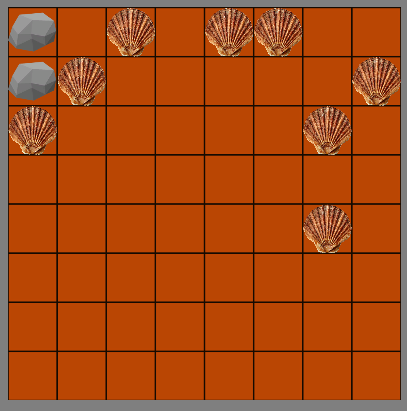
\includegraphics{img/tiefe3Hide/einkesselnHidezuhoch}
	\caption{Spielende wird nicht erkannt}
	\label{fig:nicht erkannt}
\end{figure}

\paragraph{Suchtiefe 10}
%Bei erhöhter Suchtiefe 
%% ==============================
%\section{Zusammenfassung}
%% ==============================
%\label{ch:Evaluierung:sec:zusammenfassung}

%Am Ende sollten ggf. die wichtigsten Ergebnisse nochmal in \emph{einem} kurzen Absatz zusammengefasst werden.

%%% Local Variables: 
%%% mode: latex
%%% TeX-master: "thesis"
%%% End: 
